Рассмотрим случай n поставщиков, в которой все игроки максимизируют прибыль и осведомлены о значениях базовой функциях друг друга при фиксированном бюджете K0. Для удобства пронумеруем игроков по возрастанию значению базовой функции Pi . Таким образом $P_1 \le P_2 \le \dots \le P_n$ .
Заметим, что в заданных условиях игрок n может быть уверен, что при выставлении скидки $M_{n} >P_{n-1}$он гарантированно выиграет аукцион. Тем не менее в целях максимизации математического ожидания прибыли он может быть заинтересован в выставлении меньшей скидки.
Игрок n обладает информацией о базовой функции прочих игроков, но не знает об их стратегиях выставления скидки. В условиях независимого принятия решения игроками вероятность победы в закупке $p(\Delta M_n > \Delta M_i) (i = 1, … (n-1))$ при $M_n \le P_i$ равна  $M_n/P_i$, то игрок $i$ c равной вероятностью 
выставляет скидку в меру своей базовой функции $Pi$, и $1$ при $MnPi$, конкурирующий поставщик не станет заключать сделку с отрицательной прибылью. 

Рис. 1. Вероятность предоставить для поставщика n большую скидку чем конкурент i
Fig. 1. Probability for supplier n to provide greater discount than competitor i
Следовательно математическое ожидание прибыли игрока n в введенных обозначениях запишется как:
\begin{equation}
	\mathrm{E} n(\Delta M_n) =(Pn-\Delta M_n)p(\Delta M_n>\Delta M_1,\dots,n-1)=
	(Pn-\Delta M_n)p(\Delta M_n >\Delta M_1)...p(\Delta M_n >\Delta M_n-1) 
\end{equation}


\begin{figure}[h]
    \centering
    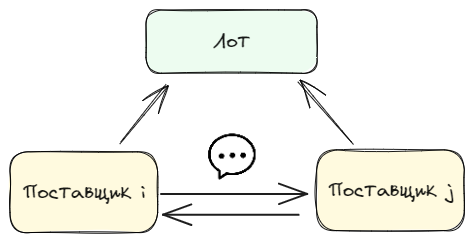
\includegraphics[width=0.5\textwidth]{assets/settings/collusion.excalidraw.png}
    \caption{Нежелательное поведение. Cговор}
\end{figure}

Полученная функция непрерывна, но не является гладкой от Mn. Имеются точки разрыва производных при значениях аргумента равных Pi. 
Предложим алгоритм поиска оптимальной скидки Mn для игрока n. Разделим поиск на два логических этапа. 
Определяем аргументы, соответствующие условному максимуму, на каждом из интервалов гладкости. На интервале $Mn \in ( Pi-1,Pi) (6) (i = 1, … (n-1), P0=0)$ запишется как:
\begin{equation}
	En =(Pn-\Delta Mn)MnPi \dots \Delta Mn Pn-1
\end{equation}	
Оптимальное значение скидки соответствует условному локальному экстремуму на множестве $M_n \in ( Pi-1,Pi)$. Выполняем дифференцирование по $M_n$ правой части уравнения 
(7) и определяем максимум на интервале:
\begin{equation}
	\begin{aligned}
		&M_n(i)=\text{arg} \max_{Mn} En= Pn(n-i)/(n-i+1),\ \text{при} Pi>Pn(n-i)/(n-i+1)> Pi-1, \\ 
		& M_n(i)=P_{i-1},\  \text{при} P_{n-i} \frac{n}{n-i+1}< Pi-1, \\
		& \Delta M_n(i)=P_i , \text{при} P_i>Pn(n-i)/(n-i+1)
	\end{aligned}
\end{equation}
Находим оптимальное значение  путем нахождения максимума конечного числа локальных максимумов, полученных на шаге 1. Оптимальное значение скидки Mn(opt)  задается как:
\begin{equation}
	M_n(opt)= \text{arg} \max_{\Delta M_1,\dots,\Delta M_n}\mathrm{E} n 
\end{equation}
Заметим, что оптимальный вид скидки $Mn(opt)$ в случае полной информированности будет определяться не только значением базовой функции поставщика $P_n$, но и соотношением между $P_1,\dots,P_n$. 
Опишем применение алгоритма для игрока $i$. Вероятность победы в закупке игрока $i$ задается как:
\begin{equation}
	\begin{cases}
		p(\Delta M_i > \Delta M_j)= \Delta M_i /Pj  если i<j \\ 
		p(\Delta Mi >\Delta Mj)= \Delta Mi/Pj при Mi<Pj  и p(\Delta Mi > \Delta Mj)=1 при MiPj  если i >j
	\end{cases}
\end{equation}
 
Аналогично математическое ожидание прибыли игрока i запишется как:
\begin{equation}
	Ei(\Delta M_i) =(Pi-\Delta M_i)p(\Delta M_i>\Delta M_1, \dots ,M_{i-1},M_{i+1},..,M_n)=
=(P_i-\Delta M_i)p(\Delta M_i >\Delta M_1) \dots p(\Delta M_i >\Delta M_n)   
\end{equation}

$Ei(\Delta M_i)$ имеет точки разрыва производных в $P_1,\dots,P_{i-1}$. Шаги оптимизационного алгоритма для игрока $i$ аналогичны поставщику n. На первом этапе выделяются максимумы на интервалах гладкости $Mi \in (0,P1) ,(P1,P2) ,\dots,(Pi-1,Pi)$. 
На втором выполняется поиск оптимального решения по конечному набору локальных максимумов, полученных на шаге 1: 
\begin{equation}
	M_i^{(opt)}= \text{arg} \max \Delta M^{(1)}i,\dots,\Delta M^{(i-1)}_i \mathrm{E}_i 
\end{equation}

Подробно разберём случай двух игроков для интерпретации результатов. Игрок с большим значением базовой функции получит номер 2 и задаст скидку:
\begin{equation}
	M_1=P_1/2 , при P_1/2 < P_2 , \text{иначе} \Delta M_1=P_2 
\end{equation}

То есть в условиях максимизации прибыли и достаточно конкурентных игроков имеем случай аналогичный закрытому аукциону. Если поставщик, обладающий значительным преимуществом, то выставляет скидку равную значению базовой функции более слабого конкурента.
Обратим внимание, что в текущей постановке задачи поставщики предполагали стратегию прочих игроков неизвестной. При максимизации выигрыша в наихудшей из возможных ситуаций получаем тривиальный вывод, что поставщик n предоставит скидку $P_{n-1}$, таким образом упуская выгоду от более рискованного предложения. 
